\section{Формализованная постановка задачи}

Во время выполнения выпускной квалификационной работы была формализована задача оценки кредитоспособности физических лиц в банковских системах с использованием алгоритма градиентного бустинга деревьев решений.

Разрабатываемое программное обеспечение предназначено для обработки входных данных заемщика, формирования признакового описания, применения обученной модели машинного обучения и получения результата скоринговой оценки.

Общая структура системы оценки кредитоспособности заемщика представлена на рисунке~\ref{fig:formal_task_0}.

\FloatBarrier
\begin{figure}[h!]
  \centering
  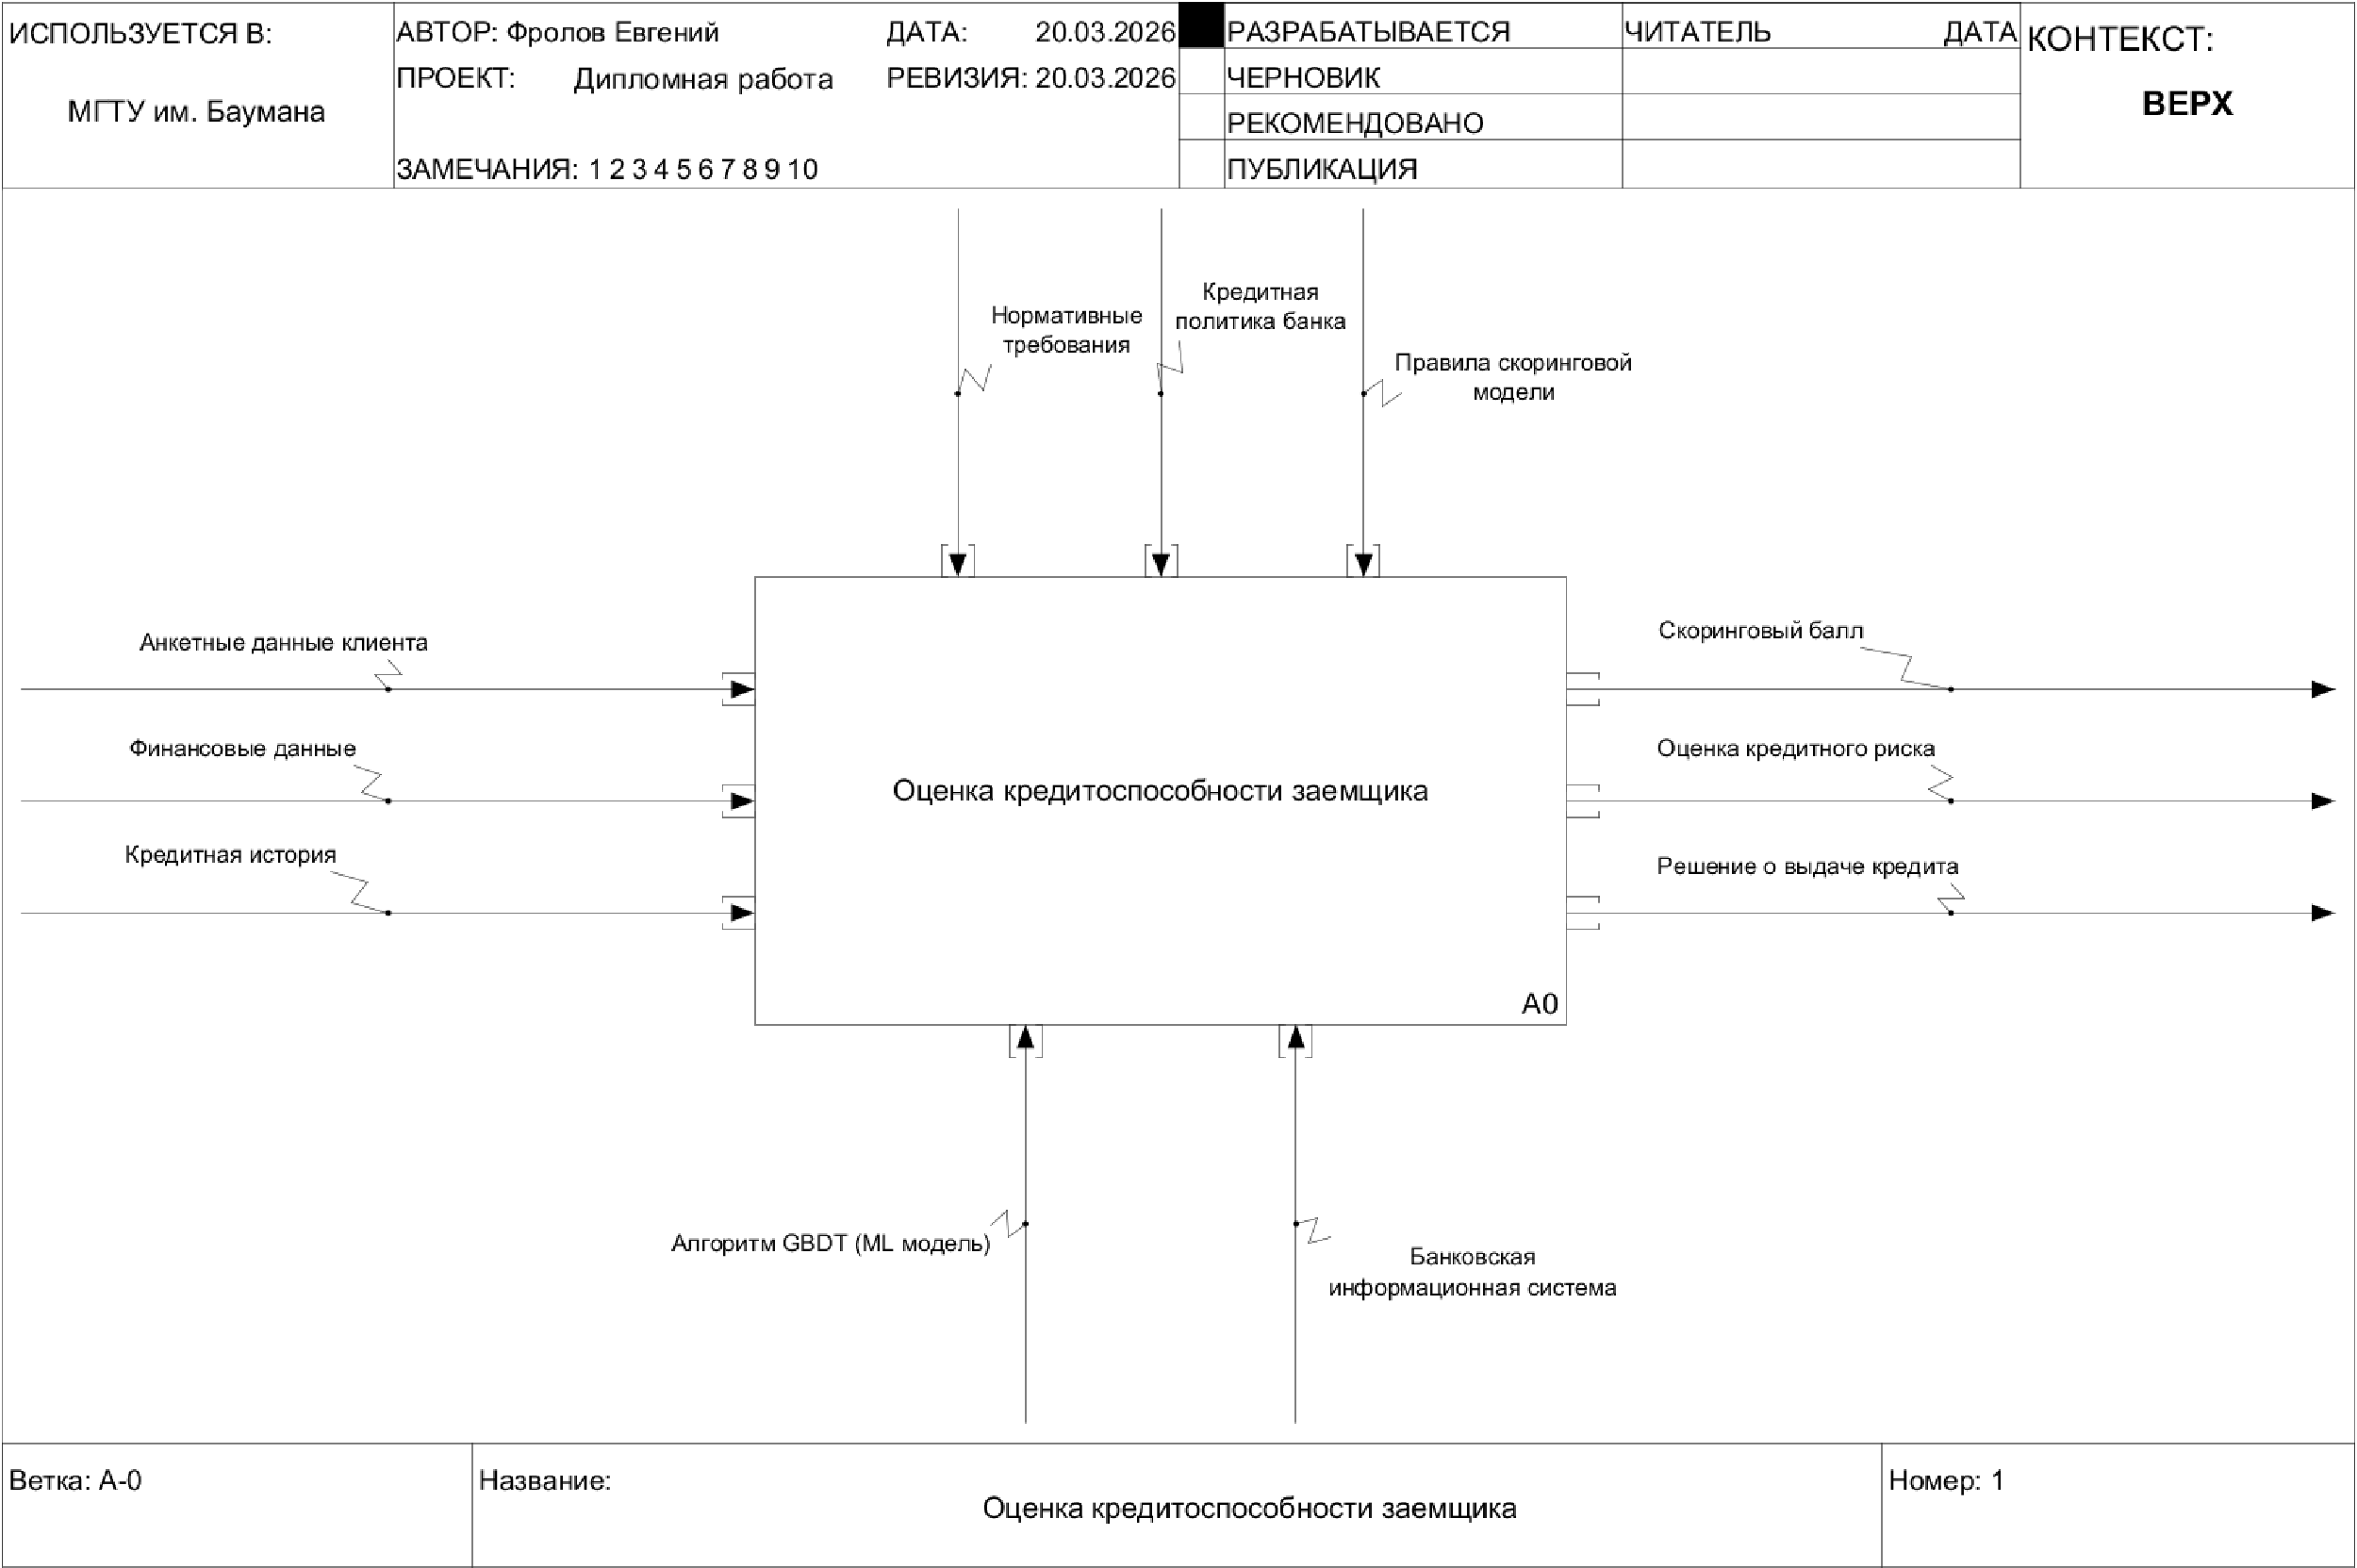
\includegraphics[width=\linewidth]{inc/pdf/01_A-0.pdf}
  \caption{IDEF0-диаграмма верхнего уровня процесса оценки кредитоспособности}
  \label{fig:formal_task_0}
\end{figure}
\FloatBarrier

На диаграмме представлены входные данные системы, управляющие воздействия, используемые механизмы и результаты работы программного комплекса.

Декомпозиция процесса оценки кредитоспособности представлена на рисунке~\ref{fig:formal_task_1}.

\FloatBarrier
\begin{figure}[h!]
  \centering
  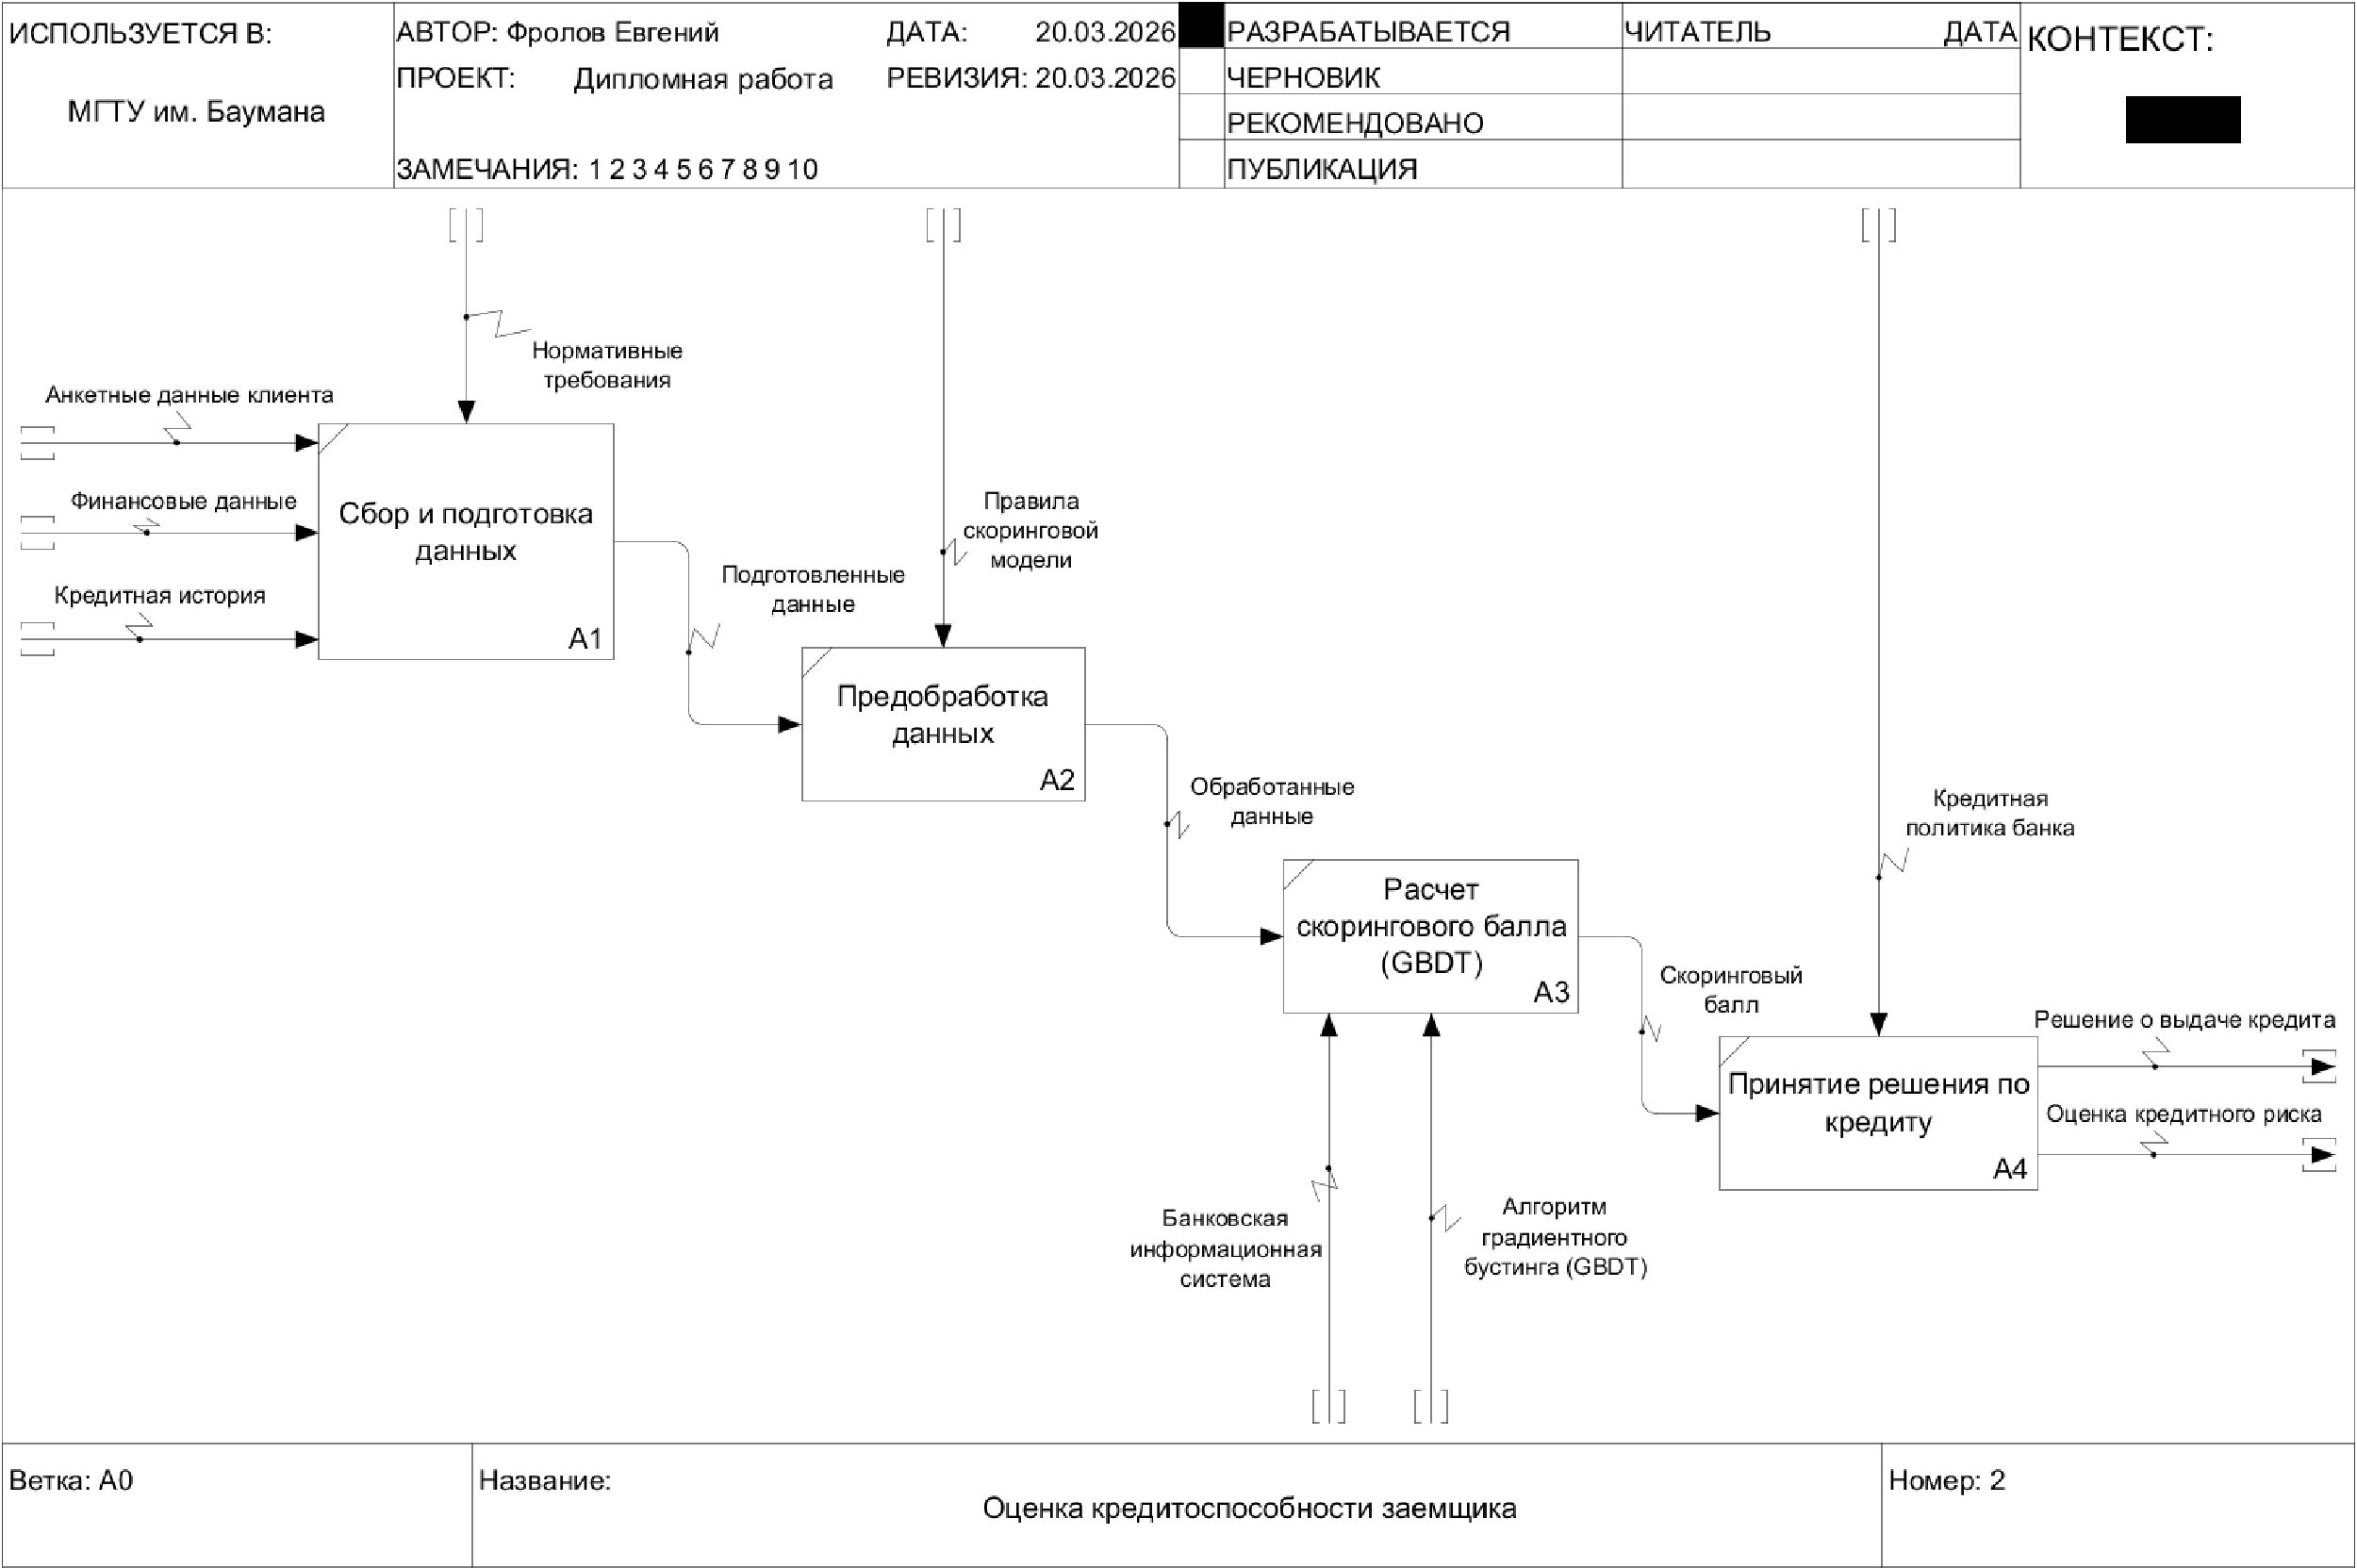
\includegraphics[width=\linewidth]{inc/pdf/02_A0.pdf}
  \caption{Декомпозиция процесса оценки кредитоспособности заемщика}
  \label{fig:formal_task_1}
\end{figure}
\FloatBarrier

Пусть задано множество заемщиков:

\begin{equation}
  D = \{(x_i, y_i)\}_{i=1}^{n},
\end{equation}

\noindent где $x_i \in \mathbb{R}^{d}$ --- вектор признаков заемщика;

\noindent\hspace*{1cm}$y_i$ --- целевая переменная;

\noindent\hspace*{1cm}$n$ --- количество объектов в выборке;

\noindent\hspace*{1cm}$d$ --- количество признаков.

Вектор признаков заемщика имеет следующий вид:

\begin{equation}
  x_i = (x_{i1}, x_{i2}, \ldots, x_{id}),
\end{equation}

\noindent где $x_{ij}$ --- значение $j$-го признака для $i$-го заемщика.

Признаковое описание заемщика формируется на основе совокупности социально-демографических, финансовых и поведенческих параметров. К ним относятся доход заемщика, сумма запрашиваемого кредита, размер ежемесячного платежа, возраст, трудовой стаж, сведения о кредитной истории, наличие просроченных платежей и информация о ранее поданных кредитных заявках.

Целевая переменная определяется следующим образом:

\begin{equation}
  y_i =
  \begin{cases}
    0, & \text{если заемщик не допустил дефолт;} \\
    1, & \text{если заемщик допустил дефолт.}
  \end{cases}
\end{equation}

Задача модели заключается в построении функции:

\begin{equation}
  f: X \rightarrow [0;1],
\end{equation}

\noindent где $X$ --- пространство признаков заемщиков.

Функция $f(x_i)$ возвращает вероятность дефолта заемщика:

\begin{equation}
  p_i = f(x_i) = P(y_i = 1 \mid x_i),
\end{equation}

\noindent где $p_i$ --- вероятность наступления дефолта для $i$-го заемщика.

На основе полученной вероятности дефолта формируется скоринговый балл:

\begin{equation}
  S_i = (1 - p_i) \cdot 1000,
\end{equation}

\noindent где $S_i$ --- скоринговый балл заемщика.

Для принятия решения используется пороговое значение вероятности дефолта:

\begin{equation}
  t = 0.5,
\end{equation}

\noindent где $t$ --- порог классификации.

Решение о принадлежности заемщика к определенному классу определяется следующим образом:

\begin{equation}
  \hat{y}_i =
  \begin{cases}
    0, & \text{если } p_i < t;    \\
    1, & \text{если } p_i \geq t.
  \end{cases}
\end{equation}

\noindent где $\hat{y}_i$ --- результат классификации заемщика.

Значение $\hat{y}_i = 0$ соответствует заемщику с низким уровнем риска, а значение $\hat{y}_i = 1$ соответствует заемщику с высоким уровнем риска дефолта.

Таким образом, задача оценки кредитоспособности физических лиц сводится к задаче бинарной классификации, в которой на основе признакового описания заемщика необходимо определить вероятность наступления дефолта и сформировать итоговое скоринговое решение.